% Author: Dun-Ming Huang
% Email: dunmingbrandonhuang@berkeley.edu
% CSM16A Fall 2022

\begin{center}
    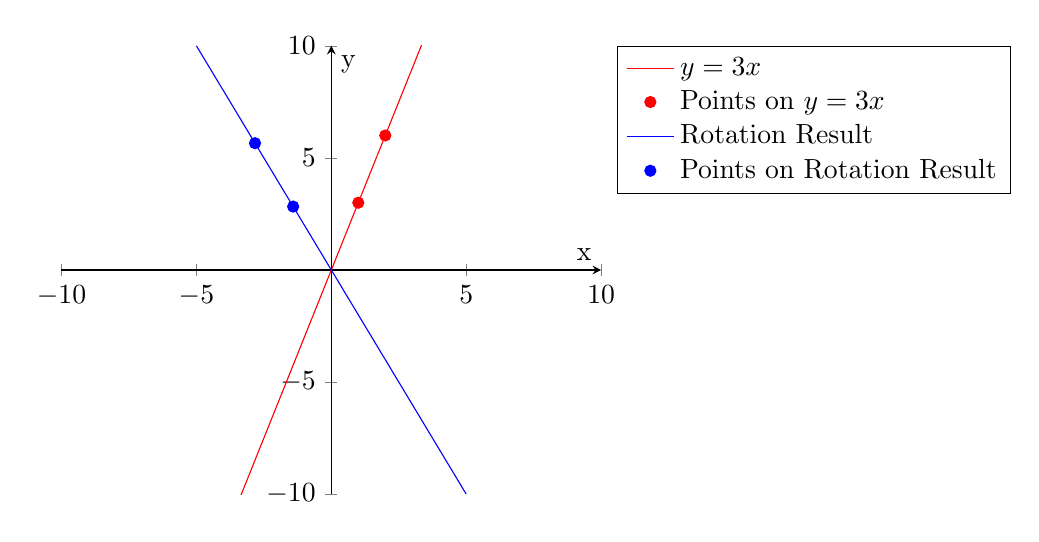
\begin{tikzpicture}
        \begin{axis}[
            axis lines = middle,
            xmin=-10, xmax=10,
            ymin=-10, ymax=10,
            xlabel = {x},
            ylabel = {y},
            legend pos=outer north east,
            legend cell align=left
        ]
            \addplot [color=red] {
               3*x
            };
            \addlegendentry{$y = 3x$}
            \addplot [only marks, color=red] table {
               1 3
               2 6
            };
            \addlegendentry{Points on $y = 3x$}
            \addplot [color=blue] {
                -2*x
            };
            \addlegendentry{Rotation Result}
            \addplot [only marks, color=blue] table {
               -1.414 2.828
               -2.828 5.656
            };
            \addlegendentry{Points on Rotation Result}
        \end{axis}
    \end{tikzpicture}
\end{center}